\documentclass[aspectratio=169]{beamer}

% Minimal theme
\usetheme{default}
\usecolortheme{dove}

% Remove navigation symbols
\setbeamertemplate{navigation symbols}{}
\setbeamertemplate{footline}{%
  \hfill{\large\insertframenumber\,/\,\inserttotalframenumber}\hspace{0.8em}\vspace{0.5em}%
}

% Colors
\definecolor{popblue}{RGB}{52, 101, 164}
\definecolor{sampred}{RGB}{204, 0, 0}
\definecolor{paramgreen}{RGB}{0, 140, 70}
\definecolor{lightbg}{RGB}{245, 245, 250}
\definecolor{warnred}{RGB}{180, 40, 40}
\definecolor{orange1}{RGB}{220, 120, 0}
\definecolor{violet1}{RGB}{120, 50, 160}

\setbeamercolor{frametitle}{fg=popblue}
\setbeamercolor{title}{fg=popblue}

% Packages
\usepackage{pgfplots}
\usepackage{tikz}
\usetikzlibrary{shapes, arrows.meta, positioning, calc, decorations.pathreplacing, patterns, fit}
\pgfplotsset{compat=1.18}
\usepackage{amsmath, amssymb}
\usepackage{array}
\usepackage{fontenc}

\title{Retrieval-Augmented Generation}
\subtitle{Embeddings $\cdot$ Vector Search $\cdot$ Chunking $\cdot$ Advanced RAG}
\date{}

\begin{document}

% ============================================================
% TITLE
% ============================================================
\begin{frame}
\titlepage
\end{frame}

% ============================================================
% WHY RAG?
% ============================================================
\begin{frame}{Why RAG?}
\begin{center}
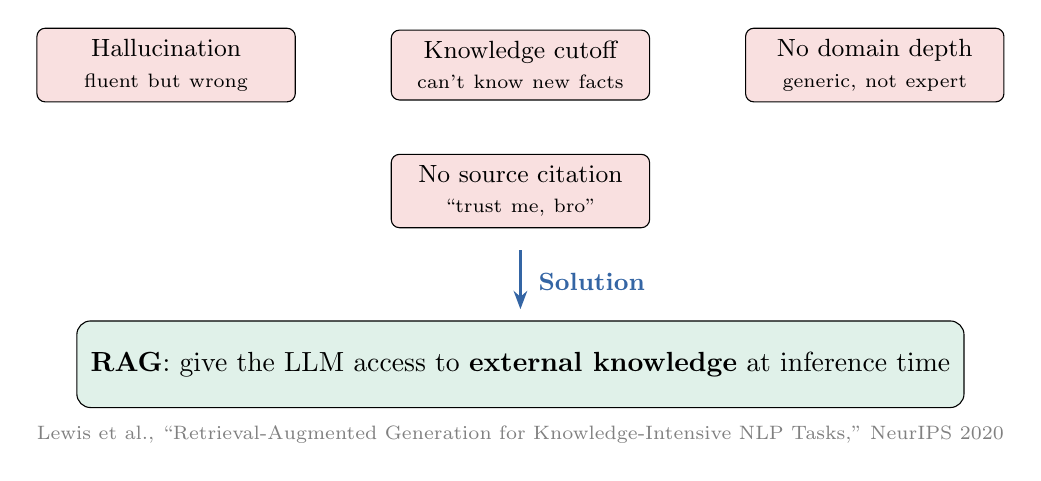
\begin{tikzpicture}[
  box/.style={draw, rounded corners=3pt, minimum width=3.2cm, minimum height=0.85cm,
              font=\small, inner sep=4pt, text width=3cm, align=center},
]
% LLM limitations
\node[box, fill=sampred!12] (hall) at (0,2.2) {Hallucination\\{\scriptsize fluent but wrong}};
\node[box, fill=sampred!12] (cutoff) at (4.5,2.2) {Knowledge cutoff\\{\scriptsize can't know new facts}};
\node[box, fill=sampred!12] (domain) at (9,2.2) {No domain depth\\{\scriptsize generic, not expert}};
\node[box, fill=sampred!12] (cite) at (4.5,0.6) {No source citation\\{\scriptsize ``trust me, bro''}};

% Arrow down
\draw[-{Stealth}, thick, popblue] (4.5,-0.15) -- (4.5,-0.9);
\node[font=\small\bfseries, popblue] at (4.5,-0.55) [right, xshift=3pt] {Solution};

% RAG box
\node[draw, rounded corners=5pt, fill=paramgreen!12, minimum width=10cm,
      minimum height=1.1cm, font=\normalsize, inner sep=5pt] (rag) at (4.5,-1.6)
      {\textbf{RAG}: give the LLM access to \textbf{external knowledge} at inference time};

% Bottom note
\node[font=\scriptsize, gray] at (4.5,-2.5)
     {Lewis et al., ``Retrieval-Augmented Generation for Knowledge-Intensive NLP Tasks,'' NeurIPS 2020};
\end{tikzpicture}
\end{center}
\end{frame}

% ============================================================
% THE BIG PICTURE
% ============================================================
\begin{frame}{The Big Picture}
\begin{center}
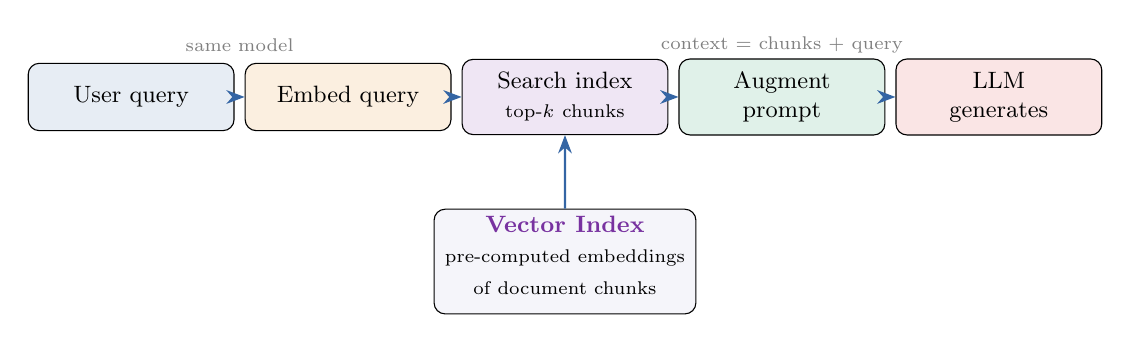
\begin{tikzpicture}[scale=0.95, transform shape,
  stp/.style={draw, rounded corners=4pt, minimum height=0.9cm, font=\small,
              inner sep=5pt, text width=2.4cm, align=center},
]
% Query phase
\node[stp, fill=popblue!12] (query) at (0,0) {User query};
\node[stp, fill=orange1!12] (embed) at (2.9,0) {Embed query};
\node[stp, fill=violet1!12] (search) at (5.8,0) {Search index\\{\scriptsize top-$k$ chunks}};
\node[stp, fill=paramgreen!12] (augment) at (8.7,0) {Augment\\prompt};
\node[stp, fill=sampred!10] (gen) at (11.6,0) {LLM\\generates};

\draw[-{Stealth}, thick, popblue] (query) -- (embed);
\draw[-{Stealth}, thick, popblue] (embed) -- (search);
\draw[-{Stealth}, thick, popblue] (search) -- (augment);
\draw[-{Stealth}, thick, popblue] (augment) -- (gen);

% Knowledge base below
\node[draw, rounded corners=4pt, fill=lightbg, minimum width=3.5cm, minimum height=1.4cm,
      font=\small, inner sep=4pt] (kb) at (5.8,-2.2) {};
\node[font=\small\bfseries, violet1] at (5.8,-1.7) {Vector Index};
\node[font=\scriptsize] at (5.8,-2.15) {pre-computed embeddings};
\node[font=\scriptsize] at (5.8,-2.55) {of document chunks};

\draw[-{Stealth}, thick, popblue] (kb) -- (search);

% Labels
\node[font=\scriptsize, gray] at (1.45, 0.7) {same model};
\node[font=\scriptsize, gray] at (8.7, 0.7) {context = chunks + query};
\end{tikzpicture}
\end{center}
\end{frame}

% ============================================================
% SPARSE VS DENSE RETRIEVAL
% ============================================================
\begin{frame}{Sparse vs Dense Retrieval}
\begin{center}
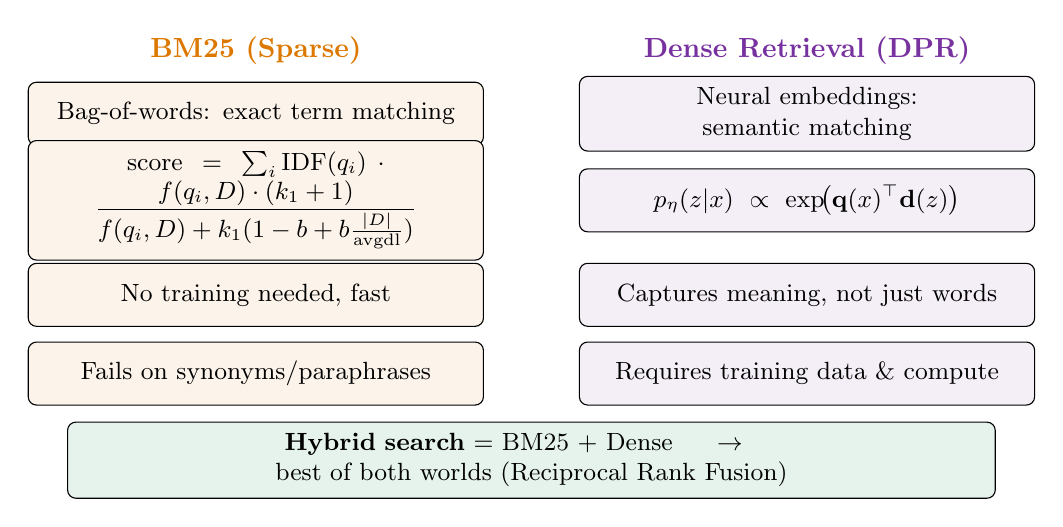
\begin{tikzpicture}[
  box/.style={draw, rounded corners=3pt, minimum height=0.8cm, font=\small,
              inner sep=4pt, text width=5.5cm, align=center},
]
% BM25 side
\node[font=\normalsize\bfseries, orange1] at (-3.5, 2.8) {BM25 (Sparse)};
\node[box, fill=orange1!8] at (-3.5, 2.0) {Bag-of-words: exact term matching};
\node[box, fill=orange1!8] at (-3.5, 0.9) {
$\text{score} = \sum_i \text{IDF}(q_i) \cdot \dfrac{f(q_i, D) \cdot (k_1+1)}{f(q_i, D) + k_1(1-b+b\tfrac{|D|}{\text{avgdl}})}$
};
\node[box, fill=orange1!8] at (-3.5, -0.3) {No training needed, fast};
\node[box, fill=orange1!8] at (-3.5, -1.3) {Fails on synonyms/paraphrases};

% Dense side
\node[font=\normalsize\bfseries, violet1] at (3.5, 2.8) {Dense Retrieval (DPR)};
\node[box, fill=violet1!8] at (3.5, 2.0) {Neural embeddings: semantic matching};
\node[box, fill=violet1!8] at (3.5, 0.9) {
$p_\eta(z|x) \propto \exp\!\bigl(\mathbf{q}(x)^\top \mathbf{d}(z)\bigr)$
};
\node[box, fill=violet1!8] at (3.5, -0.3) {Captures meaning, not just words};
\node[box, fill=violet1!8] at (3.5, -1.3) {Requires training data \& compute};

% Bottom
\node[draw, rounded corners=3pt, fill=paramgreen!10, font=\small, inner sep=4pt,
      text width=11.5cm, align=center] at (0, -2.4)
      {\textbf{Hybrid search} = BM25 + Dense $\;\to\;$ best of both worlds (Reciprocal Rank Fusion)};
\end{tikzpicture}
\end{center}
\end{frame}

% ============================================================
% EMBEDDING MODELS
% ============================================================
\begin{frame}{Embedding Models for Retrieval}
\begin{center}
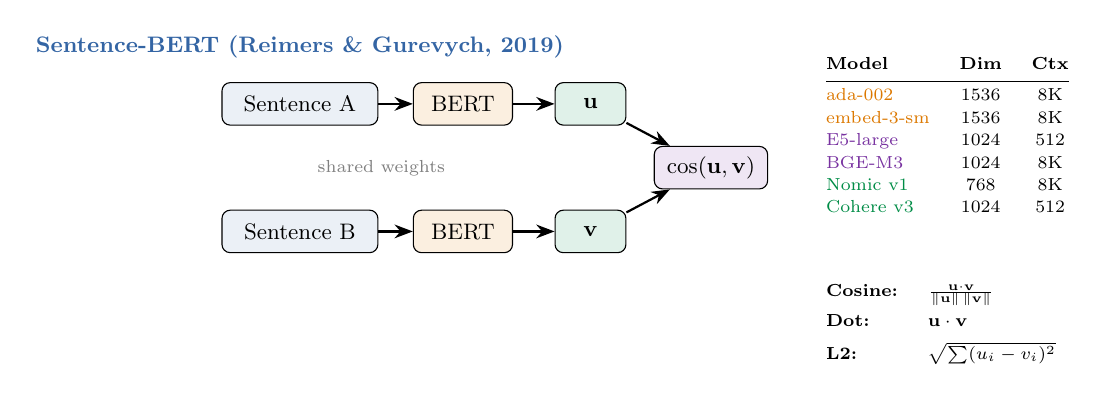
\begin{tikzpicture}[scale=0.9, transform shape]
% Siamese architecture
\node[draw, rounded corners=3pt, fill=popblue!10, minimum width=2.2cm, minimum height=0.6cm,
      font=\small] (sa) at (-2.8, 2.3) {Sentence A};
\node[draw, rounded corners=3pt, fill=popblue!10, minimum width=2.2cm, minimum height=0.6cm,
      font=\small] (sb) at (-2.8, 0.5) {Sentence B};

\node[draw, rounded corners=3pt, fill=orange1!12, minimum width=1.4cm, minimum height=0.6cm,
      font=\small] (ea) at (-0.5, 2.3) {BERT};
\node[draw, rounded corners=3pt, fill=orange1!12, minimum width=1.4cm, minimum height=0.6cm,
      font=\small] (eb) at (-0.5, 0.5) {BERT};

\node[draw, rounded corners=3pt, fill=paramgreen!12, minimum width=1cm, minimum height=0.6cm,
      font=\small] (ua) at (1.3, 2.3) {$\mathbf{u}$};
\node[draw, rounded corners=3pt, fill=paramgreen!12, minimum width=1cm, minimum height=0.6cm,
      font=\small] (ub) at (1.3, 0.5) {$\mathbf{v}$};

\node[draw, rounded corners=3pt, fill=violet1!12, minimum width=1.6cm, minimum height=0.6cm,
      font=\small] (sim) at (3, 1.4) {$\cos(\mathbf{u}, \mathbf{v})$};

\draw[-{Stealth}, thick] (sa) -- (ea);
\draw[-{Stealth}, thick] (sb) -- (eb);
\draw[-{Stealth}, thick] (ea) -- (ua);
\draw[-{Stealth}, thick] (eb) -- (ub);
\draw[-{Stealth}, thick] (ua) -- (sim);
\draw[-{Stealth}, thick] (ub) -- (sim);

\node[font=\scriptsize, gray] at (-1.65, 1.4) {shared weights};

% Label
\node[font=\small\bfseries, popblue] at (-2.8, 3.1) {Sentence-BERT (Reimers \& Gurevych, 2019)};

% Table on the right
\node[font=\scriptsize, anchor=north west] at (4.5, 3.1) {%
\begin{tabular}{@{}l c c@{}}
\textbf{Model} & \textbf{Dim} & \textbf{Ctx} \\[2pt]
\hline\\[-6pt]
\color{orange1}{ada-002} & 1536 & 8K \\[1pt]
\color{orange1}{embed-3-sm} & 1536 & 8K \\[1pt]
\color{violet1}{E5-large} & 1024 & 512 \\[1pt]
\color{violet1}{BGE-M3} & 1024 & 8K \\[1pt]
\color{paramgreen}{Nomic v1} & 768 & 8K \\[1pt]
\color{paramgreen}{Cohere v3} & 1024 & 512 \\[1pt]
\end{tabular}};

% Similarity formulas below
\node[font=\scriptsize, anchor=north west] at (4.5, -0.1) {%
\begin{tabular}{@{}l l@{}}
\textbf{Cosine:} & $\frac{\mathbf{u} \cdot \mathbf{v}}{\|\mathbf{u}\|\,\|\mathbf{v}\|}$ \\[4pt]
\textbf{Dot:} & $\mathbf{u} \cdot \mathbf{v}$ \\[4pt]
\textbf{L2:} & $\sqrt{\sum(u_i - v_i)^2}$ \\
\end{tabular}};

\end{tikzpicture}
\end{center}
\end{frame}

% ============================================================
% CONTRASTIVE TRAINING
% ============================================================
\begin{frame}{Contrastive Training for Embeddings}
\begin{center}
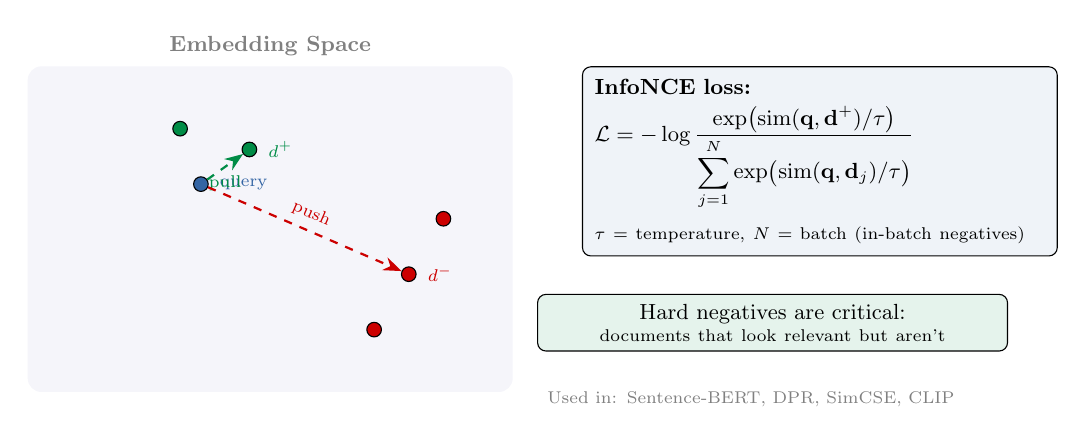
\begin{tikzpicture}[scale=0.88, transform shape,
  pt/.style={circle, draw, minimum size=6pt, inner sep=0pt},
]
% Embedding space
\fill[lightbg, rounded corners=5pt] (-2.5,-2.2) rectangle (4.5,2.5);
\node[font=\small\bfseries, gray] at (1,2.8) {Embedding Space};

% Positive cluster
\node[pt, fill=popblue] (q) at (0,0.8) {};
\node[font=\scriptsize, popblue, right] at (0.15,0.8) {query};
\node[pt, fill=paramgreen] (p1) at (0.7,1.3) {};
\node[font=\scriptsize, paramgreen, right] at (0.85,1.3) {$d^+$};
\node[pt, fill=paramgreen] (p2) at (-0.3,1.6) {};

% Negative points
\node[pt, fill=sampred] (n1) at (3.0,-0.5) {};
\node[pt, fill=sampred] (n2) at (3.5,0.3) {};
\node[pt, fill=sampred] (n3) at (2.5,-1.3) {};
\node[font=\scriptsize, sampred, right] at (3.15,-0.5) {$d^-$};

% Arrows
\draw[-{Stealth}, paramgreen, thick, dashed] (q) -- (p1) node[midway, below, font=\scriptsize] {pull};
\draw[-{Stealth}, sampred, thick, dashed] (q) -- (n1) node[midway, above, font=\scriptsize, sloped] {push};

% InfoNCE loss on the right
\node[draw, rounded corners=3pt, fill=popblue!8, inner sep=5pt,
      text width=6.5cm, align=left, font=\small, anchor=north west] (loss) at (5.5, 2.5)
{
\textbf{InfoNCE loss:}\\[4pt]
$\mathcal{L} = -\log \dfrac{\exp\bigl(\text{sim}(\mathbf{q}, \mathbf{d}^+)/\tau\bigr)}{\displaystyle\sum_{j=1}^{N}\exp\bigl(\text{sim}(\mathbf{q}, \mathbf{d}_j)/\tau\bigr)}$
\\[6pt]
{\scriptsize $\tau$ = temperature, $N$ = batch (in-batch negatives)}
};

% Key idea box
\node[draw, rounded corners=3pt, fill=paramgreen!10, inner sep=4pt,
      text width=6.5cm, align=center, font=\small] at (8.25, -1.2)
{Hard negatives are critical:\\[-2pt]
{\scriptsize documents that look relevant but aren't}};

% Examples
\node[font=\scriptsize, gray, text width=6.5cm, align=left] at (8.25, -2.3)
{Used in: Sentence-BERT, DPR, SimCSE, CLIP};
\end{tikzpicture}
\end{center}
\end{frame}

% ============================================================
% VECTOR DATABASES
% ============================================================
\begin{frame}{Vector Databases \& ANN Search}
\begin{center}
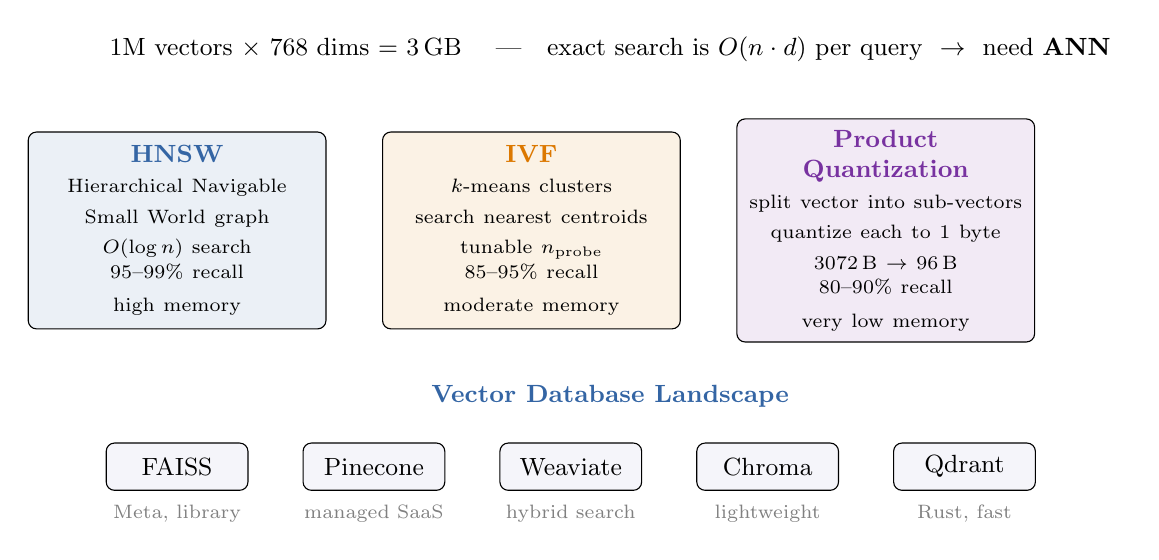
\begin{tikzpicture}[
  box/.style={draw, rounded corners=3pt, font=\small, inner sep=4pt, align=center},
]
% Problem statement
\node[font=\small, text width=13cm, align=center] at (5.5, 2.8)
{1M vectors $\times$ 768 dims $=$ 3\,GB \quad---\quad exact search is $O(n \cdot d)$ per query $\;\to\;$ need \textbf{ANN}};

% Three ANN methods
\node[box, fill=popblue!10, text width=3.5cm, minimum height=2.5cm] (hnsw) at (0, 0.5)
{\textbf{\color{popblue}HNSW}\\[3pt]
{\scriptsize Hierarchical Navigable\\Small World graph}\\[3pt]
{\scriptsize $O(\log n)$ search\\[1pt]
95--99\% recall\\[1pt]
high memory}};

\node[box, fill=orange1!10, text width=3.5cm, minimum height=2.5cm] (ivf) at (4.5, 0.5)
{\textbf{\color{orange1}IVF}\\[3pt]
{\scriptsize $k$-means clusters\\search nearest centroids}\\[3pt]
{\scriptsize tunable $n_\text{probe}$\\[1pt]
85--95\% recall\\[1pt]
moderate memory}};

\node[box, fill=violet1!10, text width=3.5cm, minimum height=2.5cm] (pq) at (9, 0.5)
{\textbf{\color{violet1}Product Quantization}\\[3pt]
{\scriptsize split vector into sub-vectors\\quantize each to 1 byte}\\[3pt]
{\scriptsize 3072\,B $\to$ 96\,B\\[1pt]
80--90\% recall\\[1pt]
very low memory}};

% DB landscape
\node[font=\small\bfseries, popblue] at (5.5, -1.6) {Vector Database Landscape};

\node[box, fill=lightbg, minimum width=1.8cm, minimum height=0.6cm] (faiss) at (0, -2.5) {FAISS};
\node[box, fill=lightbg, minimum width=1.8cm, minimum height=0.6cm] (pine) at (2.5, -2.5) {Pinecone};
\node[box, fill=lightbg, minimum width=1.8cm, minimum height=0.6cm] (weav) at (5, -2.5) {Weaviate};
\node[box, fill=lightbg, minimum width=1.8cm, minimum height=0.6cm] (chro) at (7.5, -2.5) {Chroma};
\node[box, fill=lightbg, minimum width=1.8cm, minimum height=0.6cm] (qdr) at (10, -2.5) {Qdrant};

\node[font=\scriptsize, gray] at (0, -3.1) {Meta, library};
\node[font=\scriptsize, gray] at (2.5, -3.1) {managed SaaS};
\node[font=\scriptsize, gray] at (5, -3.1) {hybrid search};
\node[font=\scriptsize, gray] at (7.5, -3.1) {lightweight};
\node[font=\scriptsize, gray] at (10, -3.1) {Rust, fast};
\end{tikzpicture}
\end{center}
\end{frame}

% ============================================================
% CHUNKING STRATEGIES
% ============================================================
\begin{frame}{Chunking Strategies}
\begin{center}
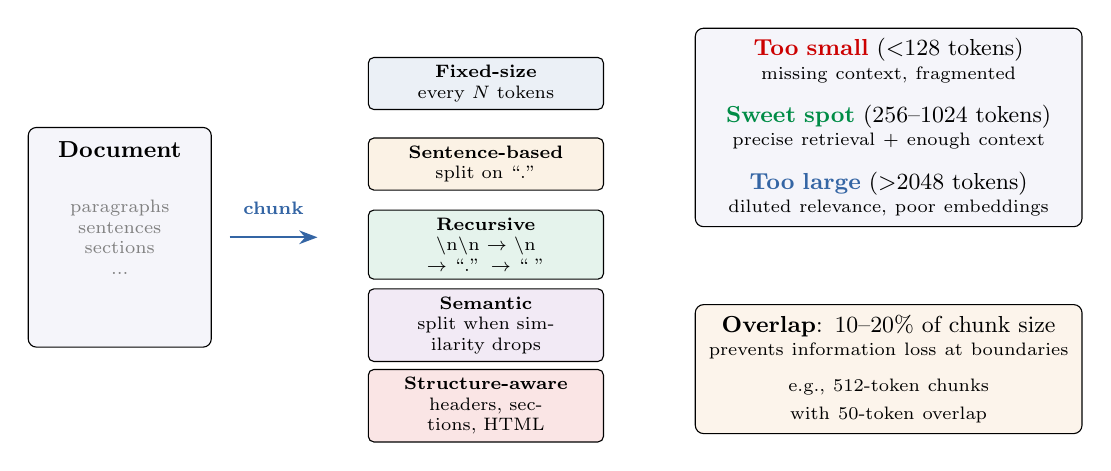
\begin{tikzpicture}[scale=0.93, transform shape,
  chunk/.style={draw, rounded corners=2pt, font=\scriptsize, inner sep=3pt,
                minimum height=0.55cm, align=center},
]
% Document on the left
\node[draw, rounded corners=3pt, fill=lightbg, minimum width=2.5cm, minimum height=3cm,
      font=\small, inner sep=4pt] (doc) at (-1.5, 0.5) {};
\node[font=\small\bfseries] at (-1.5, 1.7) {Document};
\node[font=\scriptsize, gray, text width=2cm, align=center] at (-1.5, 0.5)
     {paragraphs\\sentences\\sections\\...};

% Arrow
\draw[-{Stealth}, thick, popblue] (0, 0.5) -- (1.2, 0.5);
\node[font=\scriptsize\bfseries, popblue] at (0.6, 0.9) {chunk};

% Strategies
\node[chunk, fill=popblue!10, text width=3cm] (fix) at (3.5, 2.6) {\textbf{Fixed-size}\\every $N$ tokens};
\node[chunk, fill=orange1!10, text width=3cm] (sent) at (3.5, 1.5) {\textbf{Sentence-based}\\split on ``.''};
\node[chunk, fill=paramgreen!10, text width=3cm] (recur) at (3.5, 0.4) {\textbf{Recursive}\\{\scriptsize \textbackslash n\textbackslash n $\to$ \textbackslash n $\to$ ``.'' $\to$ `` ''}};
\node[chunk, fill=violet1!10, text width=3cm] (sem) at (3.5, -0.7) {\textbf{Semantic}\\{\scriptsize split when similarity drops}};
\node[chunk, fill=sampred!10, text width=3cm] (struct) at (3.5, -1.8) {\textbf{Structure-aware}\\{\scriptsize headers, sections, HTML}};

% Trade-off on the right
\node[draw, rounded corners=3pt, fill=lightbg, inner sep=4pt, text width=5cm,
      align=center, font=\small] at (9, 2) {
\textbf{\color{sampred}Too small} ($<$128 tokens)\\[-2pt]
{\scriptsize missing context, fragmented}\\[6pt]
\textbf{\color{paramgreen}Sweet spot} (256--1024 tokens)\\[-2pt]
{\scriptsize precise retrieval + enough context}\\[6pt]
\textbf{\color{popblue}Too large} ($>$2048 tokens)\\[-2pt]
{\scriptsize diluted relevance, poor embeddings}
};

% Overlap note
\node[draw, rounded corners=3pt, fill=orange1!8, inner sep=4pt, text width=5cm,
      align=center, font=\small] at (9, -1.3)
{\textbf{Overlap}: 10--20\% of chunk size\\[-2pt]
{\scriptsize prevents information loss at boundaries}\\[3pt]
{\scriptsize e.g., 512-token chunks with 50-token overlap}};
\end{tikzpicture}
\end{center}
\end{frame}

% ============================================================
% THE INDEXING PIPELINE
% ============================================================
\begin{frame}{Phase 1: Indexing (Offline)}
\begin{center}
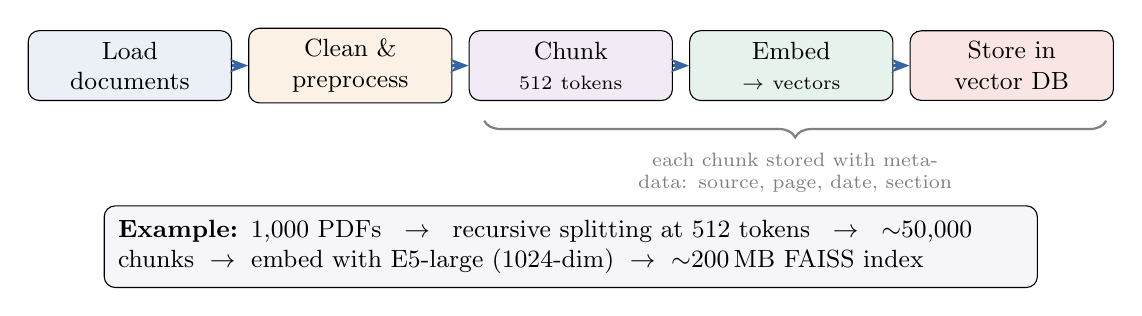
\begin{tikzpicture}[
  stp/.style={draw, rounded corners=4pt, minimum height=0.85cm, font=\small,
              inner sep=4pt, text width=2.3cm, align=center},
]
\node[stp, fill=popblue!10] (docs) at (0,0) {Load\\documents};
\node[stp, fill=orange1!10] (clean) at (2.8,0) {Clean \&\\preprocess};
\node[stp, fill=violet1!10] (chk) at (5.6,0) {Chunk\\{\scriptsize 512 tokens}};
\node[stp, fill=paramgreen!10] (emb) at (8.4,0) {Embed\\{\scriptsize $\to$ vectors}};
\node[stp, fill=sampred!10] (store) at (11.2,0) {Store in\\vector DB};

\draw[-{Stealth}, thick, popblue] (docs) -- (clean);
\draw[-{Stealth}, thick, popblue] (clean) -- (chk);
\draw[-{Stealth}, thick, popblue] (chk) -- (emb);
\draw[-{Stealth}, thick, popblue] (emb) -- (store);

% Metadata annotation
\draw[decorate, decoration={brace, amplitude=6pt, mirror}, thick, gray]
     (4.5,-0.7) -- (12.4,-0.7) node[midway, below=8pt, font=\scriptsize, gray, text width=6cm, align=center]
     {each chunk stored with metadata: source, page, date, section};

% Concrete example
\node[draw, rounded corners=4pt, fill=lightbg, inner sep=5pt, text width=11.5cm,
      align=left, font=\small] at (5.6, -2.3)
{\textbf{Example:} 1{,}000 PDFs $\;\to\;$ recursive splitting at 512 tokens $\;\to\;$ $\sim$50{,}000 chunks
$\;\to\;$ embed with E5-large (1024-dim) $\;\to\;$ $\sim$200\,MB FAISS index};
\end{tikzpicture}
\end{center}
\end{frame}

% ============================================================
% THE QUERY PIPELINE
% ============================================================
\begin{frame}{Phase 2: Query (Online)}
\begin{center}
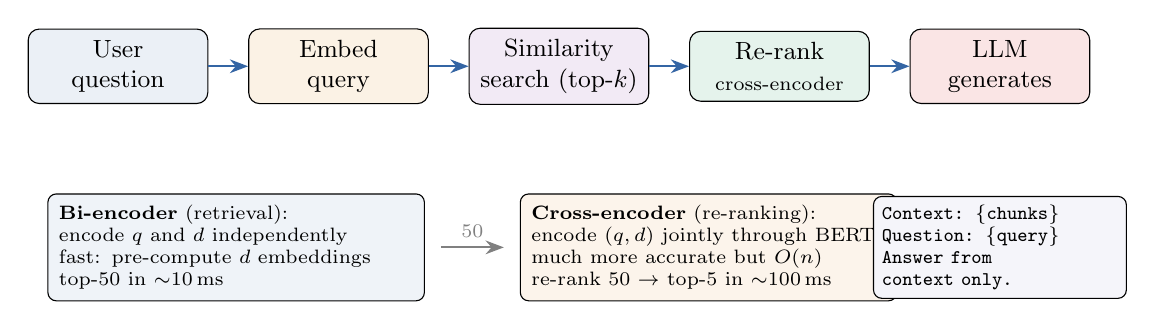
\begin{tikzpicture}[
  stp/.style={draw, rounded corners=4pt, minimum height=0.8cm, font=\small,
              inner sep=4pt, align=center},
]
% Main flow
\node[stp, fill=popblue!10, text width=2cm] (q) at (0, 1) {User\\question};
\node[stp, fill=orange1!10, text width=2cm] (emb) at (2.8, 1) {Embed\\query};
\node[stp, fill=violet1!10, text width=2cm] (sim) at (5.6, 1) {Similarity\\search (top-$k$)};
\node[stp, fill=paramgreen!10, text width=2cm] (rerank) at (8.4, 1) {Re-rank\\{\scriptsize cross-encoder}};
\node[stp, fill=sampred!10, text width=2cm] (gen) at (11.2, 1) {LLM\\generates};

\draw[-{Stealth}, thick, popblue] (q) -- (emb);
\draw[-{Stealth}, thick, popblue] (emb) -- (sim);
\draw[-{Stealth}, thick, popblue] (sim) -- (rerank);
\draw[-{Stealth}, thick, popblue] (rerank) -- (gen);

% Bi-encoder vs cross-encoder
\node[draw, rounded corners=3pt, fill=popblue!8, inner sep=4pt, text width=4.5cm,
      align=left, font=\scriptsize] at (1.5, -1.3)
{\textbf{Bi-encoder} (retrieval):\\
encode $q$ and $d$ independently\\
fast: pre-compute $d$ embeddings\\
top-50 in $\sim$10\,ms};

\node[draw, rounded corners=3pt, fill=orange1!8, inner sep=4pt, text width=4.5cm,
      align=left, font=\scriptsize] at (7.5, -1.3)
{\textbf{Cross-encoder} (re-ranking):\\
encode $(q, d)$ jointly through BERT\\
much more accurate but $O(n)$\\
re-rank 50 $\to$ top-5 in $\sim$100\,ms};

% Arrow between them
\draw[-{Stealth}, thick, gray] (4.1, -1.3) -- (4.9, -1.3)
     node[midway, above, font=\scriptsize, gray] {50};

% Prompt template
\node[draw, rounded corners=3pt, fill=lightbg, inner sep=3pt, text width=3cm,
      align=left, font=\scriptsize] at (11.2, -1.3)
{\texttt{Context: \{chunks\}}\\
\texttt{Question: \{query\}}\\
\texttt{Answer from}\\
\texttt{context only.}};
\end{tikzpicture}
\end{center}
\end{frame}

% ============================================================
% HYBRID SEARCH & RRF
% ============================================================
\begin{frame}{Hybrid Search \& Reciprocal Rank Fusion}
\begin{center}
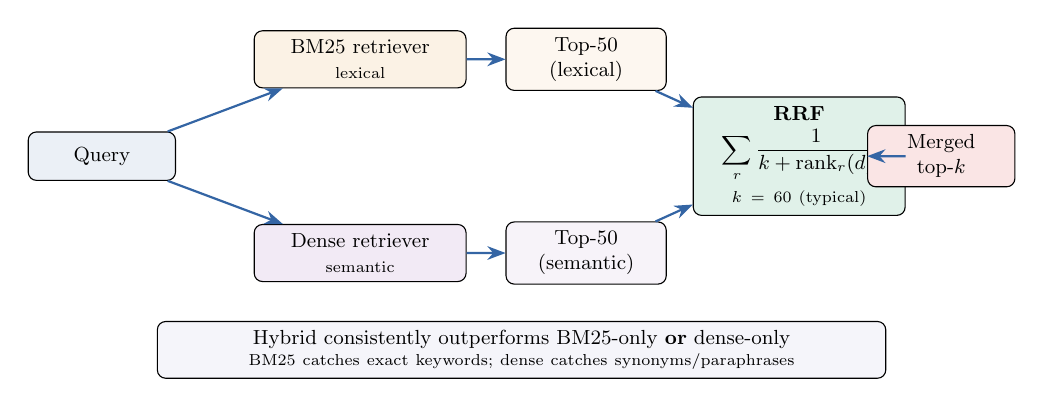
\begin{tikzpicture}[scale=0.82, transform shape,
  box/.style={draw, rounded corners=3pt, minimum height=0.75cm, font=\small,
              inner sep=4pt, align=center},
]
% Query
\node[box, fill=popblue!10, text width=2cm] (q) at (0, 0) {Query};

% Two paths
\node[box, fill=orange1!10, text width=3cm] (bm) at (4, 1.5) {BM25 retriever\\{\scriptsize lexical}};
\node[box, fill=violet1!10, text width=3cm] (dn) at (4, -1.5) {Dense retriever\\{\scriptsize semantic}};

\draw[-{Stealth}, thick, popblue] (q) -- (bm);
\draw[-{Stealth}, thick, popblue] (q) -- (dn);

% Results
\node[box, fill=orange1!6, text width=2.2cm] (r1) at (7.5, 1.5) {Top-50\\(lexical)};
\node[box, fill=violet1!6, text width=2.2cm] (r2) at (7.5, -1.5) {Top-50\\(semantic)};

\draw[-{Stealth}, thick, popblue] (bm) -- (r1);
\draw[-{Stealth}, thick, popblue] (dn) -- (r2);

% RRF
\node[box, fill=paramgreen!12, text width=3cm, minimum height=1.5cm] (rrf) at (10.8, 0)
{\textbf{RRF}\\[3pt]
$\displaystyle\sum_r \frac{1}{k + \text{rank}_r(d)}$\\[3pt]
{\scriptsize $k = 60$ (typical)}};

\draw[-{Stealth}, thick, popblue] (r1) -- (rrf);
\draw[-{Stealth}, thick, popblue] (r2) -- (rrf);

% Output
\node[box, fill=sampred!10, text width=2cm] (out) at (13, 0) {Merged\\top-$k$};
\draw[-{Stealth}, thick, popblue] (rrf) -- (out);

% Bottom note
\node[draw, rounded corners=3pt, fill=lightbg, inner sep=4pt, text width=11cm,
      align=center, font=\small] at (6.5, -3)
{Hybrid consistently outperforms BM25-only \textbf{or} dense-only\\[-2pt]
{\scriptsize BM25 catches exact keywords; dense catches synonyms/paraphrases}};
\end{tikzpicture}
\end{center}
\end{frame}

% ============================================================
% THE ORIGINAL RAG PAPER
% ============================================================
\begin{frame}{The Original RAG Paper (Lewis et al., 2020)}
\begin{center}
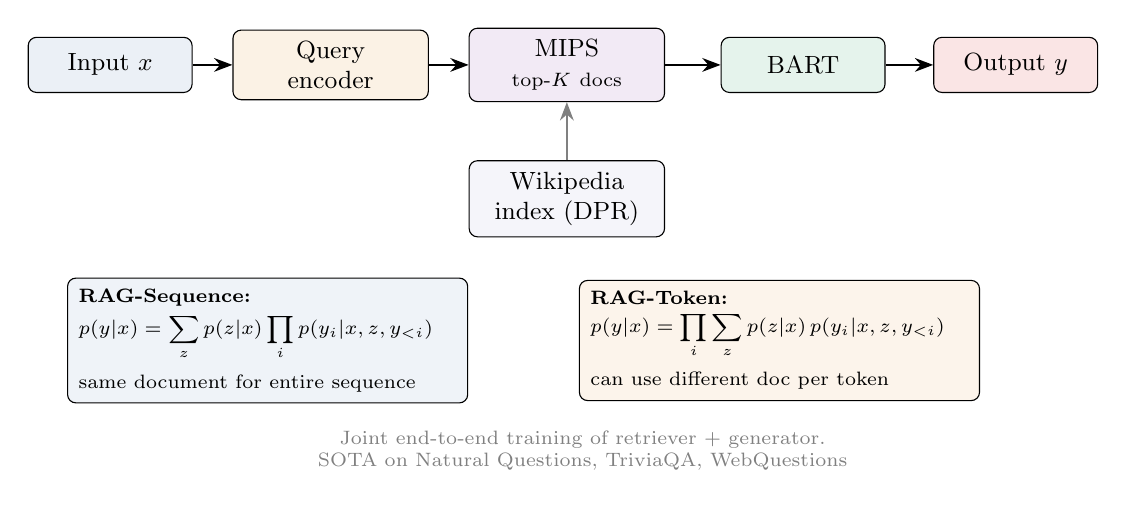
\begin{tikzpicture}[
  box/.style={draw, rounded corners=3pt, minimum height=0.7cm, font=\small,
              inner sep=4pt, align=center},
]
% Architecture
\node[box, fill=popblue!10, text width=1.8cm] (input) at (0, 1.5) {Input $x$};
\node[box, fill=orange1!10, text width=2.2cm] (qenc) at (2.8, 1.5) {Query\\encoder};
\node[box, fill=violet1!10, text width=2.2cm] (mips) at (5.8, 1.5) {MIPS\\{\scriptsize top-$K$ docs}};
\node[box, fill=paramgreen!10, text width=1.8cm] (bart) at (8.8, 1.5) {BART};
\node[box, fill=sampred!10, text width=1.8cm] (out) at (11.5, 1.5) {Output $y$};

\draw[-{Stealth}, thick] (input) -- (qenc);
\draw[-{Stealth}, thick] (qenc) -- (mips);
\draw[-{Stealth}, thick] (mips) -- (bart);
\draw[-{Stealth}, thick] (bart) -- (out);

% Wikipedia index
\node[box, fill=lightbg, text width=2.2cm] (wiki) at (5.8, -0.2) {Wikipedia\\index (DPR)};
\draw[-{Stealth}, thick, gray] (wiki) -- (mips);

% RAG-Sequence vs RAG-Token
\node[draw, rounded corners=3pt, fill=popblue!8, inner sep=4pt, text width=4.8cm,
      align=left, font=\scriptsize] at (2, -2)
{\textbf{RAG-Sequence:}\\[2pt]
$p(y|x) = \displaystyle\sum_z p(z|x)\prod_i p(y_i|x,z,y_{<i})$\\[4pt]
same document for entire sequence};

\node[draw, rounded corners=3pt, fill=orange1!8, inner sep=4pt, text width=4.8cm,
      align=left, font=\scriptsize] at (8.5, -2)
{\textbf{RAG-Token:}\\[2pt]
$p(y|x) = \displaystyle\prod_i \sum_z p(z|x)\, p(y_i|x,z,y_{<i})$\\[4pt]
can use different doc per token};

% Bottom
\node[font=\scriptsize, gray, text width=12cm, align=center] at (6, -3.4)
{Joint end-to-end training of retriever + generator.
SOTA on Natural Questions, TriviaQA, WebQuestions};
\end{tikzpicture}
\end{center}
\end{frame}

% ============================================================
% QUERY TRANSFORMATION: HyDE
% ============================================================
\begin{frame}{Query Transformation: HyDE}
\begin{center}
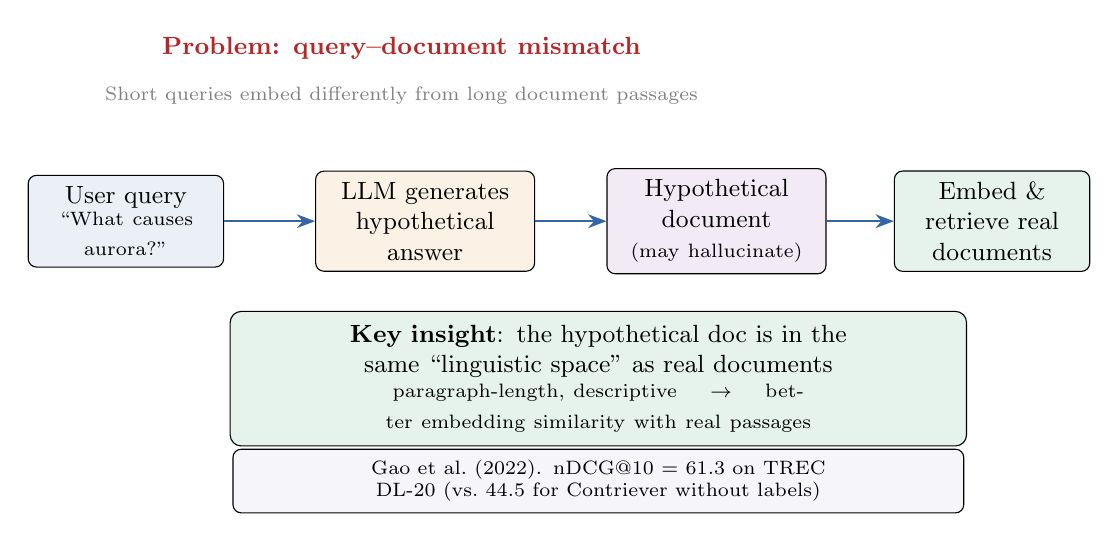
\begin{tikzpicture}[
  box/.style={draw, rounded corners=3pt, minimum height=0.7cm, font=\small,
              inner sep=4pt, align=center},
]
% Problem
\node[font=\small\bfseries, warnred] at (2, 3) {Problem: query--document mismatch};
\node[font=\scriptsize, gray, text width=8cm, align=center] at (2, 2.4)
{Short queries embed differently from long document passages};

% Pipeline
\node[box, fill=popblue!10, text width=2.2cm] (q) at (-1.5, 0.8) {User query\\{\scriptsize ``What causes\\aurora?''}};
\node[box, fill=orange1!10, text width=2.5cm] (llm) at (2.3, 0.8) {LLM generates\\hypothetical\\answer};
\node[box, fill=violet1!10, text width=2.5cm] (hyp) at (6, 0.8) {Hypothetical\\document\\{\scriptsize (may hallucinate)}};
\node[box, fill=paramgreen!10, text width=2.2cm] (emb) at (9.5, 0.8) {Embed \&\\retrieve real\\documents};

\draw[-{Stealth}, thick, popblue] (q) -- (llm);
\draw[-{Stealth}, thick, popblue] (llm) -- (hyp);
\draw[-{Stealth}, thick, popblue] (hyp) -- (emb);

% Key insight
\node[draw, rounded corners=4pt, fill=paramgreen!10, inner sep=5pt, text width=9cm,
      align=center, font=\small] at (4.5, -1.2)
{\textbf{Key insight}: the hypothetical doc is in the same ``linguistic space''
as real documents\\[-2pt]
{\scriptsize paragraph-length, descriptive $\;\to\;$ better embedding similarity with real passages}};

% Results
\node[draw, rounded corners=3pt, fill=lightbg, inner sep=4pt, text width=9cm,
      align=center, font=\scriptsize] at (4.5, -2.5)
{Gao et al.\ (2022). nDCG@10 = 61.3 on TREC DL-20 (vs.\ 44.5 for Contriever without labels)};
\end{tikzpicture}
\end{center}
\end{frame}

% ============================================================
% PARENT-CHILD CHUNKING
% ============================================================
\begin{frame}{Parent-Child Chunking}
\begin{center}
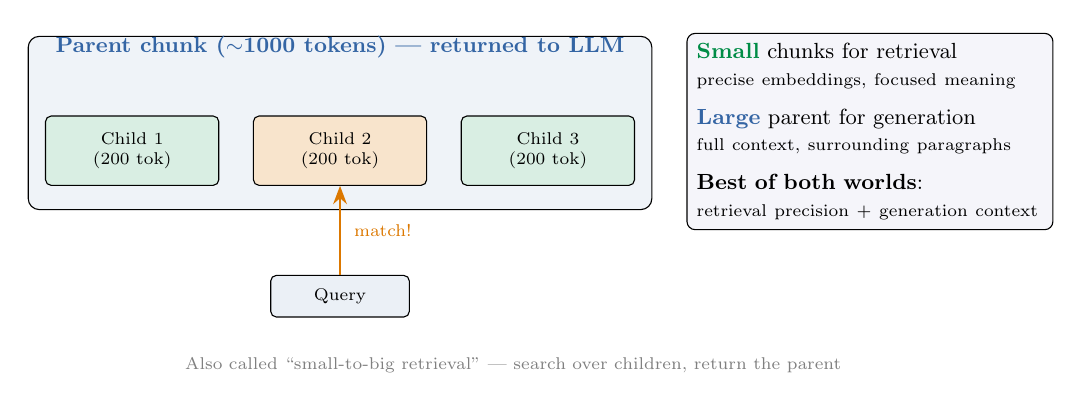
\begin{tikzpicture}[scale=0.88, transform shape,
  box/.style={draw, rounded corners=2pt, font=\scriptsize, inner sep=3pt, align=center},
]
% Parent chunk
\node[draw, rounded corners=4pt, fill=popblue!8, minimum width=9cm, minimum height=2.5cm,
      inner sep=4pt] (parent) at (0, 0.7) {};
\node[font=\small\bfseries, popblue] at (0, 1.8) {Parent chunk ($\sim$1000 tokens) --- returned to LLM};

% Child chunks inside
\node[box, fill=paramgreen!15, minimum width=2.5cm, minimum height=1cm]
     (c1) at (-3, 0.3) {Child 1\\(200 tok)};
\node[box, fill=orange1!20, minimum width=2.5cm, minimum height=1cm]
     (c2) at (0, 0.3) {Child 2\\(200 tok)};
\node[box, fill=paramgreen!15, minimum width=2.5cm, minimum height=1cm]
     (c3) at (3, 0.3) {Child 3\\(200 tok)};

% Query matches child 2
\node[box, fill=popblue!10, minimum width=2cm, minimum height=0.6cm]
     (query) at (0, -1.8) {Query};
\draw[-{Stealth}, thick, orange1] (query) -- (c2)
     node[midway, right, font=\scriptsize, orange1, xshift=2pt] {match!};

% Explanation
\node[draw, rounded corners=3pt, fill=lightbg, inner sep=4pt, text width=5cm,
      align=left, font=\small, anchor=north west] at (5, 2)
{
\textbf{\color{paramgreen}Small} chunks for retrieval\\
{\scriptsize precise embeddings, focused meaning}\\[5pt]
\textbf{\color{popblue}Large} parent for generation\\
{\scriptsize full context, surrounding paragraphs}\\[5pt]
\textbf{Best of both worlds}:\\
{\scriptsize retrieval precision + generation context}
};

% Bottom note
\node[font=\scriptsize, gray, text width=12cm, align=center] at (2.5, -2.8)
{Also called ``small-to-big retrieval'' --- search over children, return the parent};
\end{tikzpicture}
\end{center}
\end{frame}

% ============================================================
% SELF-RAG
% ============================================================
\begin{frame}{Self-RAG (Asai et al., 2023)}
\begin{center}
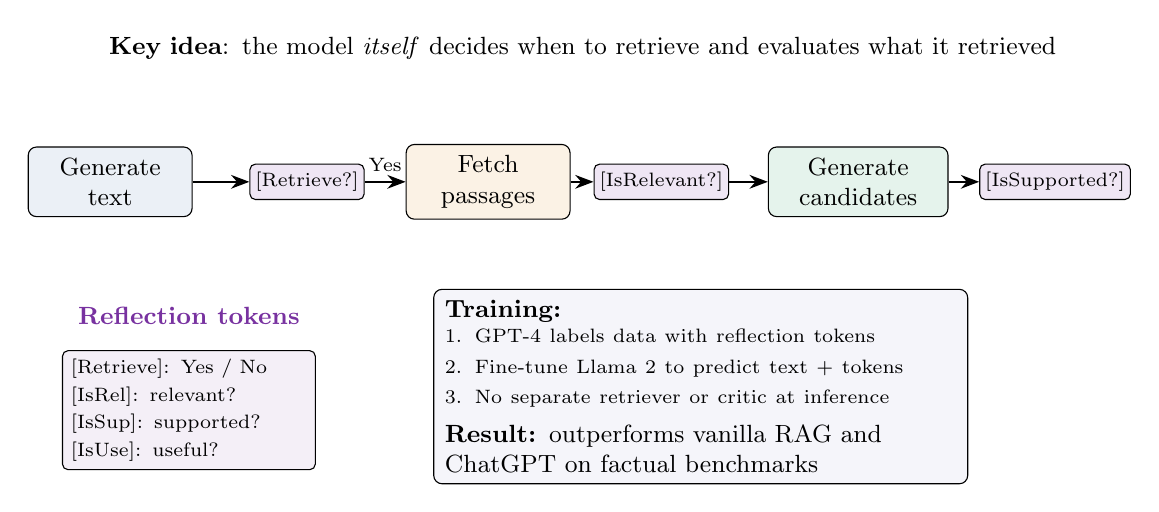
\begin{tikzpicture}[
  box/.style={draw, rounded corners=3pt, minimum height=0.6cm, font=\small,
              inner sep=4pt, align=center},
  tok/.style={draw, rounded corners=2pt, font=\scriptsize, inner sep=2pt,
              minimum height=0.45cm, fill=violet1!12},
]
% Idea
\node[font=\small, text width=13cm, align=center] at (6, 2.9)
{\textbf{Key idea}: the model \emph{itself} decides when to retrieve and evaluates what it retrieved};

% Flow
\node[box, fill=popblue!10, text width=1.8cm] (gen1) at (0, 1.2) {Generate\\text};
\node[tok] (ret) at (2.5, 1.2) {[Retrieve?]};
\node[box, fill=orange1!10, text width=1.8cm] (fetch) at (4.8, 1.2) {Fetch\\passages};
\node[tok] (rel) at (7, 1.2) {[IsRelevant?]};
\node[box, fill=paramgreen!10, text width=2cm] (gen2) at (9.5, 1.2) {Generate\\candidates};
\node[tok] (sup) at (12, 1.2) {[IsSupported?]};

\draw[-{Stealth}, thick] (gen1) -- (ret);
\draw[-{Stealth}, thick] (ret) -- (fetch) node[midway, above, font=\scriptsize] {Yes};
\draw[-{Stealth}, thick] (fetch) -- (rel);
\draw[-{Stealth}, thick] (rel) -- (gen2);
\draw[-{Stealth}, thick] (gen2) -- (sup);

% Reflection tokens
\node[font=\small\bfseries, violet1] at (1, -0.5) {Reflection tokens};

\node[draw, rounded corners=2pt, fill=violet1!8, inner sep=3pt, text width=3cm,
      align=left, font=\scriptsize] at (1, -1.7)
{[Retrieve]: Yes / No\\[2pt]
[IsRel]: relevant?\\[2pt]
[IsSup]: supported?\\[2pt]
[IsUse]: useful?};

% Training
\node[draw, rounded corners=3pt, fill=lightbg, inner sep=4pt, text width=6.5cm,
      align=left, font=\small] at (7.5, -1.4)
{\textbf{Training:}\\[-2pt]
{\scriptsize 1. GPT-4 labels data with reflection tokens}\\
{\scriptsize 2. Fine-tune Llama 2 to predict text + tokens}\\
{\scriptsize 3. No separate retriever or critic at inference}\\[3pt]
\textbf{Result:} outperforms vanilla RAG and\\
ChatGPT on factual benchmarks};
\end{tikzpicture}
\end{center}
\end{frame}

% ============================================================
% CORRECTIVE RAG
% ============================================================
\begin{frame}{Corrective RAG (Yan et al., 2024)}
\begin{center}
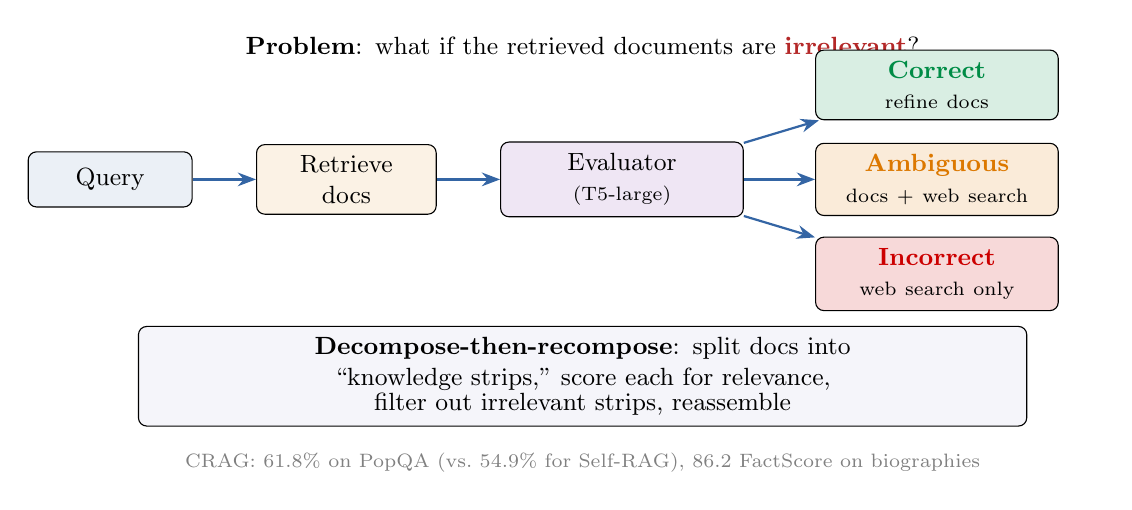
\begin{tikzpicture}[
  box/.style={draw, rounded corners=3pt, minimum height=0.7cm, font=\small,
              inner sep=4pt, align=center},
]
% Problem
\node[font=\small, text width=13cm, align=center] at (6, 3)
{\textbf{Problem}: what if the retrieved documents are \textbf{\color{warnred}irrelevant}?};

% Flow
\node[box, fill=popblue!10, text width=1.8cm] (q) at (0, 1.3) {Query};
\node[box, fill=orange1!10, text width=2cm] (ret) at (3, 1.3) {Retrieve\\docs};
\node[box, fill=violet1!12, text width=2.8cm] (eval) at (6.5, 1.3) {Evaluator\\{\scriptsize (T5-large)}};

\draw[-{Stealth}, thick, popblue] (q) -- (ret);
\draw[-{Stealth}, thick, popblue] (ret) -- (eval);

% Three branches
\node[box, fill=paramgreen!15, text width=2.8cm] (correct) at (10.5, 2.5)
{\textbf{\color{paramgreen}Correct}\\{\scriptsize refine docs}};
\node[box, fill=orange1!15, text width=2.8cm] (ambig) at (10.5, 1.3)
{\textbf{\color{orange1}Ambiguous}\\{\scriptsize docs + web search}};
\node[box, fill=sampred!15, text width=2.8cm] (wrong) at (10.5, 0.1)
{\textbf{\color{sampred}Incorrect}\\{\scriptsize web search only}};

\draw[-{Stealth}, thick, popblue] (eval) -- (correct);
\draw[-{Stealth}, thick, popblue] (eval) -- (ambig);
\draw[-{Stealth}, thick, popblue] (eval) -- (wrong);

% Decompose-then-recompose
\node[draw, rounded corners=3pt, fill=lightbg, inner sep=4pt, text width=11cm,
      align=center, font=\small] at (6, -1.2)
{\textbf{Decompose-then-recompose}: split docs into ``knowledge strips,''
score each for relevance,\\[-2pt]
filter out irrelevant strips, reassemble};

% Results
\node[font=\scriptsize, gray, text width=11cm, align=center] at (6, -2.3)
{CRAG: 61.8\% on PopQA (vs.\ 54.9\% for Self-RAG), 86.2 FactScore on biographies};
\end{tikzpicture}
\end{center}
\end{frame}

% ============================================================
% LOST IN THE MIDDLE
% ============================================================
\begin{frame}{Lost in the Middle (Liu et al., 2023)}
\vspace{-0.4cm}
\begin{center}
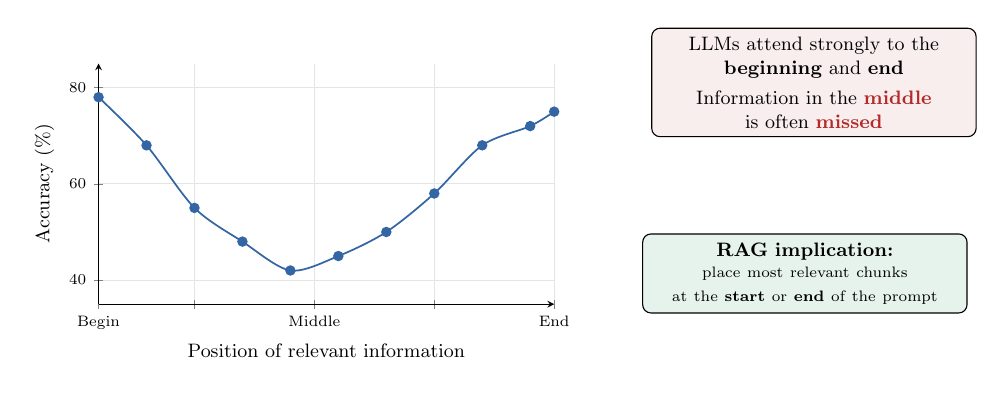
\begin{tikzpicture}[scale=0.78, transform shape]
% U-shaped curve
\begin{axis}[
  width=9cm, height=5.5cm,
  xlabel={Position of relevant information},
  ylabel={Accuracy (\%)},
  xtick={1,5,10,15,20},
  xticklabels={Begin, , Middle, , End},
  ymin=35, ymax=85,
  axis lines=left,
  xlabel style={font=\small},
  ylabel style={font=\small},
  tick label style={font=\scriptsize},
  grid=major,
  grid style={gray!20},
]
\addplot[thick, popblue, mark=*, mark size=2pt, smooth]
  coordinates {(1,78) (3,68) (5,55) (7,48) (9,42) (11,45) (13,50) (15,58) (17,68) (19,72) (20,75)};
\end{axis}

% Annotation
\node[draw, rounded corners=3pt, fill=warnred!8, inner sep=4pt, text width=5cm,
      align=center, font=\small, anchor=north west] at (9, 4.5)
{LLMs attend strongly to the\\
\textbf{beginning} and \textbf{end}\\[3pt]
Information in the \textbf{\color{warnred}middle}\\
is often \textbf{\color{warnred}missed}};

% Practical implication
\node[draw, rounded corners=3pt, fill=paramgreen!10, inner sep=4pt, text width=5cm,
      align=center, font=\small] at (11.5, 0.5)
{\textbf{RAG implication:}\\[2pt]
{\scriptsize place most relevant chunks\\
at the \textbf{start} or \textbf{end} of the prompt}};
\end{tikzpicture}
\end{center}
\end{frame}

% ============================================================
% RAG VS FINE-TUNING
% ============================================================
\begin{frame}{RAG vs Fine-Tuning}
\begin{center}
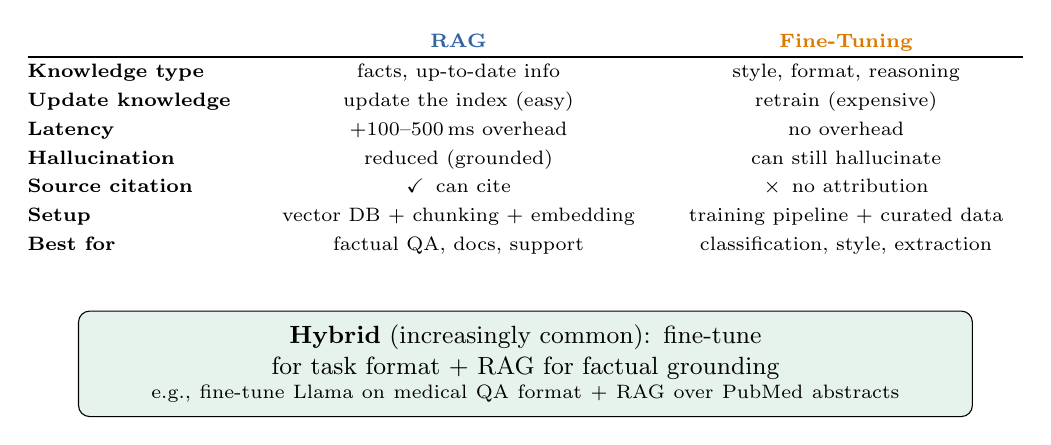
\begin{tikzpicture}
\node[font=\scriptsize, inner sep=0pt] at (6.5, 0) {%
\renewcommand{\arraystretch}{1.3}%
\begin{tabular}{@{} >{\raggedright}p{2.8cm} >{\centering}p{4.5cm} >{\centering\arraybackslash}p{4.5cm} @{}}
& \textbf{\color{popblue}RAG} & \textbf{\color{orange1}Fine-Tuning} \\
\hline
\textbf{Knowledge type} & facts, up-to-date info & style, format, reasoning \\
\textbf{Update knowledge} & update the index (easy) & retrain (expensive) \\
\textbf{Latency} & +100--500\,ms overhead & no overhead \\
\textbf{Hallucination} & reduced (grounded) & can still hallucinate \\
\textbf{Source citation} & $\checkmark$\, can cite & $\times$\, no attribution \\
\textbf{Setup} & vector DB + chunking + embedding & training pipeline + curated data \\
\textbf{Best for} & factual QA, docs, support & classification, style, extraction \\
\end{tabular}};

% Bottom: hybrid
\node[draw, rounded corners=4pt, fill=paramgreen!10, inner sep=5pt, text width=11cm,
      align=center, font=\small] at (6.5, -2.8)
{\textbf{Hybrid} (increasingly common): fine-tune for task format + RAG for factual grounding\\[-2pt]
{\scriptsize e.g., fine-tune Llama on medical QA format + RAG over PubMed abstracts}};
\end{tikzpicture}
\end{center}
\end{frame}

% ============================================================
% EVALUATION: RAGAS
% ============================================================
\begin{frame}{Evaluating RAG: RAGAS Framework}
\begin{center}
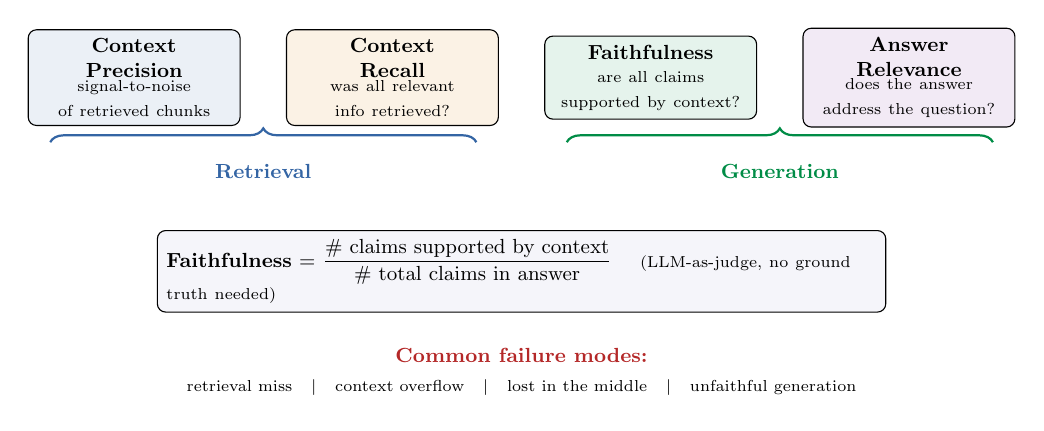
\begin{tikzpicture}[scale=0.82, transform shape,
  box/.style={draw, rounded corners=3pt, minimum height=1.1cm, font=\small,
              inner sep=4pt, align=center, text width=3cm},
]
% Four metrics
\node[box, fill=popblue!10] (cp) at (0, 1.5) {\textbf{Context}\\
\textbf{Precision}\\[-2pt]
{\scriptsize signal-to-noise\\of retrieved chunks}};

\node[box, fill=orange1!10] (cr) at (4, 1.5) {\textbf{Context}\\
\textbf{Recall}\\[-2pt]
{\scriptsize was all relevant\\info retrieved?}};

\node[box, fill=paramgreen!10] (faith) at (8, 1.5) {\textbf{Faithfulness}\\[2pt]
{\scriptsize are all claims\\supported by context?}};

\node[box, fill=violet1!10] (rel) at (12, 1.5) {\textbf{Answer}\\
\textbf{Relevance}\\[-2pt]
{\scriptsize does the answer\\address the question?}};

% Braces
\draw[decorate, decoration={brace, amplitude=5pt}, thick, popblue]
     (-1.3, 0.5) -- (5.3, 0.5) node[midway, below=6pt, font=\small\bfseries, popblue] {Retrieval};
\draw[decorate, decoration={brace, amplitude=5pt}, thick, paramgreen]
     (6.7, 0.5) -- (13.3, 0.5) node[midway, below=6pt, font=\small\bfseries, paramgreen] {Generation};

% Faithfulness formula
\node[draw, rounded corners=3pt, fill=lightbg, inner sep=4pt, text width=11cm,
      align=left, font=\small] at (6, -1.5)
{\textbf{Faithfulness} = $\dfrac{\text{\# claims supported by context}}{\text{\# total claims in answer}}$
\quad{\scriptsize (LLM-as-judge, no ground truth needed)}};

% Failure modes
\node[font=\small\bfseries, warnred] at (6, -2.8) {Common failure modes:};
\node[font=\scriptsize, text width=12cm, align=center] at (6, -3.3)
{retrieval miss $\;\mid\;$ context overflow $\;\mid\;$ lost in the middle $\;\mid\;$ unfaithful generation};
\end{tikzpicture}
\end{center}
\end{frame}

% ============================================================
% LATENCY & PRACTICAL CONSIDERATIONS
% ============================================================
\begin{frame}{Practical Considerations}
\vspace{-0.3cm}
\begin{center}
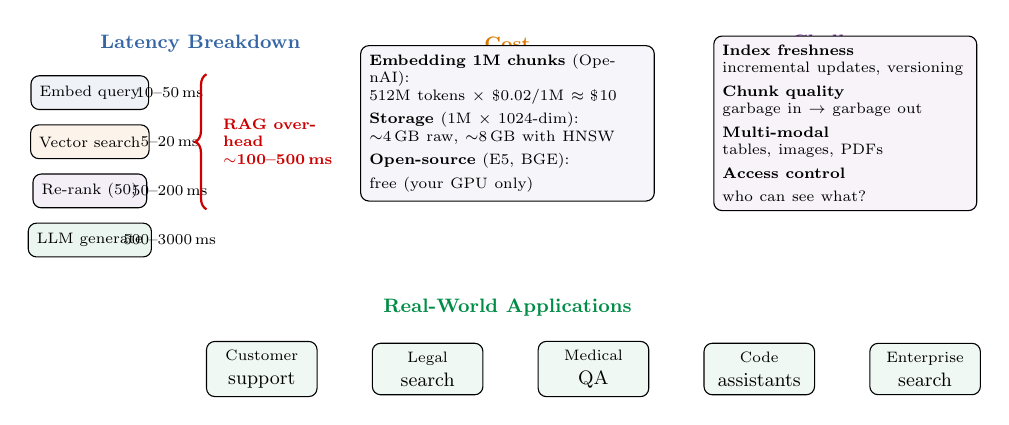
\begin{tikzpicture}[scale=0.78, transform shape,
  box/.style={draw, rounded corners=3pt, font=\small, inner sep=4pt, align=center},
]
% Latency breakdown
\node[font=\small\bfseries, popblue] at (-1.5, 2.8) {Latency Breakdown};

\node[box, fill=popblue!8, minimum width=1.2cm, minimum height=0.55cm] at (-3.3, 2)
{\scriptsize Embed query};
\node[font=\scriptsize] at (-2, 2) {10--50\,ms};

\node[box, fill=orange1!8, minimum width=1.2cm, minimum height=0.55cm] at (-3.3, 1.2)
{\scriptsize Vector search};
\node[font=\scriptsize] at (-2, 1.2) {5--20\,ms};

\node[box, fill=violet1!8, minimum width=1.2cm, minimum height=0.55cm] at (-3.3, 0.4)
{\scriptsize Re-rank (50)};
\node[font=\scriptsize] at (-2, 0.4) {50--200\,ms};

\node[box, fill=paramgreen!8, minimum width=1.2cm, minimum height=0.55cm] at (-3.3, -0.4)
{\scriptsize LLM generate};
\node[font=\scriptsize] at (-2, -0.4) {500--3000\,ms};

\draw[thick, sampred, decorate, decoration={brace, amplitude=4pt, mirror}]
     (-1.4, 2.3) -- (-1.4, 0.1)
     node[midway, right=4pt, font=\scriptsize\bfseries, sampred, text width=2cm] {RAG overhead\\$\sim$100--500\,ms};

% Cost column
\node[font=\small\bfseries, orange1] at (3.5, 2.8) {Cost};

\node[box, fill=lightbg, text width=4.5cm, align=left] at (3.5, 1.5)
{{\scriptsize
\textbf{Embedding 1M chunks} (OpenAI):\\
512M tokens $\times$ \$0.02/1M $\approx$ \$10\\[3pt]
\textbf{Storage} (1M $\times$ 1024-dim):\\
$\sim$4\,GB raw, $\sim$8\,GB with HNSW\\[3pt]
\textbf{Open-source} (E5, BGE):\\
free (your GPU only)}};

% Challenges column
\node[font=\small\bfseries, violet1] at (9, 2.8) {Challenges};

\node[box, fill=violet1!6, text width=4cm, align=left] at (9, 1.5)
{{\scriptsize
\textbf{Index freshness}\\
incremental updates, versioning\\[3pt]
\textbf{Chunk quality}\\
garbage in $\to$ garbage out\\[3pt]
\textbf{Multi-modal}\\
tables, images, PDFs\\[3pt]
\textbf{Access control}\\
who can see what?}};

% Applications at bottom
\node[font=\small\bfseries, paramgreen] at (3.5, -1.5) {Real-World Applications};

\node[box, fill=paramgreen!6, minimum width=1.8cm, minimum height=0.5cm]
     at (-0.5, -2.5) {\scriptsize Customer\\support};
\node[box, fill=paramgreen!6, minimum width=1.8cm, minimum height=0.5cm]
     at (2.2, -2.5) {\scriptsize Legal\\search};
\node[box, fill=paramgreen!6, minimum width=1.8cm, minimum height=0.5cm]
     at (4.9, -2.5) {\scriptsize Medical\\QA};
\node[box, fill=paramgreen!6, minimum width=1.8cm, minimum height=0.5cm]
     at (7.6, -2.5) {\scriptsize Code\\assistants};
\node[box, fill=paramgreen!6, minimum width=1.8cm, minimum height=0.5cm]
     at (10.3, -2.5) {\scriptsize Enterprise\\search};
\end{tikzpicture}
\end{center}
\end{frame}

% ============================================================
% RAG EVOLUTION
% ============================================================
\begin{frame}{RAG Evolution}
\begin{center}
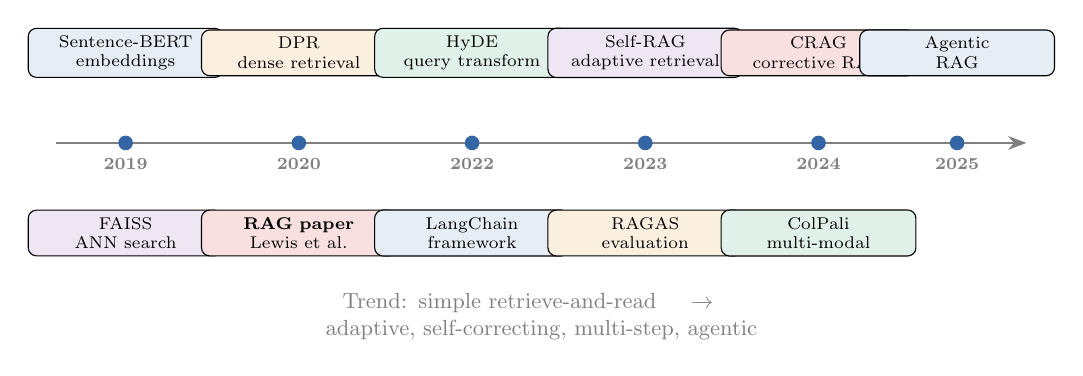
\begin{tikzpicture}[scale=0.88, transform shape,
  evt/.style={draw, rounded corners=3pt, font=\scriptsize, inner sep=3pt,
              text width=2.6cm, align=center, minimum height=0.55cm},
]
% Timeline axis
\draw[thick, -Stealth, gray] (0, 0) -- (14, 0);

% Year markers
\node[font=\scriptsize\bfseries, gray, below] at (1, -0.1) {2019};
\node[font=\scriptsize\bfseries, gray, below] at (3.5, -0.1) {2020};
\node[font=\scriptsize\bfseries, gray, below] at (6, -0.1) {2022};
\node[font=\scriptsize\bfseries, gray, below] at (8.5, -0.1) {2023};
\node[font=\scriptsize\bfseries, gray, below] at (11, -0.1) {2024};
\node[font=\scriptsize\bfseries, gray, below] at (13, -0.1) {2025};

% Events above
\node[evt, fill=popblue!12] at (1, 1.3) {Sentence-BERT\\embeddings};
\node[evt, fill=orange1!12] at (3.5, 1.3) {DPR\\dense retrieval};
\node[evt, fill=paramgreen!12] at (6, 1.3) {HyDE\\query transform};
\node[evt, fill=violet1!12] at (8.5, 1.3) {Self-RAG\\adaptive retrieval};
\node[evt, fill=sampred!12] at (11, 1.3) {CRAG\\corrective RAG};
\node[evt, fill=popblue!12] at (13, 1.3) {Agentic\\RAG};

% Events below
\node[evt, fill=violet1!12] at (1, -1.3) {FAISS\\ANN search};
\node[evt, fill=sampred!12] at (3.5, -1.3) {\textbf{RAG paper}\\Lewis et al.};
\node[evt, fill=popblue!12] at (6, -1.3) {LangChain\\framework};
\node[evt, fill=orange1!12] at (8.5, -1.3) {RAGAS\\evaluation};
\node[evt, fill=paramgreen!12] at (11, -1.3) {ColPali\\multi-modal};

% Dots on timeline
\fill[popblue] (1, 0) circle (3pt);
\fill[popblue] (3.5, 0) circle (3pt);
\fill[popblue] (6, 0) circle (3pt);
\fill[popblue] (8.5, 0) circle (3pt);
\fill[popblue] (11, 0) circle (3pt);
\fill[popblue] (13, 0) circle (3pt);

% Trend arrow
\node[font=\small, gray, text width=10cm, align=center] at (7, -2.5)
{Trend: simple retrieve-and-read $\;\to\;$ adaptive, self-correcting, multi-step, agentic};
\end{tikzpicture}
\end{center}
\end{frame}

% ============================================================
% SUMMARY
% ============================================================
\begin{frame}{The RAG Playbook}
\begin{center}
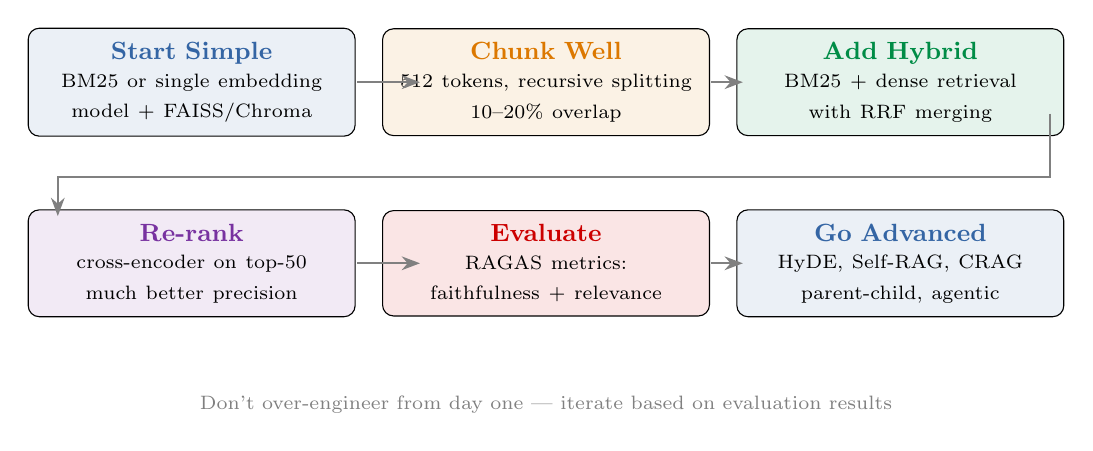
\begin{tikzpicture}[
  card/.style={draw, rounded corners=4pt, font=\small, inner sep=5pt,
               text width=3.8cm, align=center, minimum height=1.3cm},
]
\node[card, fill=popblue!10] at (0, 1.8)
{\textbf{\color{popblue}Start Simple}\\[2pt]
{\scriptsize BM25 or single embedding\\model + FAISS/Chroma}};

\node[card, fill=orange1!10] at (4.5, 1.8)
{\textbf{\color{orange1}Chunk Well}\\[2pt]
{\scriptsize 512 tokens, recursive splitting\\10--20\% overlap}};

\node[card, fill=paramgreen!10] at (9, 1.8)
{\textbf{\color{paramgreen}Add Hybrid}\\[2pt]
{\scriptsize BM25 + dense retrieval\\with RRF merging}};

\node[card, fill=violet1!10] at (0, -0.5)
{\textbf{\color{violet1}Re-rank}\\[2pt]
{\scriptsize cross-encoder on top-50\\much better precision}};

\node[card, fill=sampred!10] at (4.5, -0.5)
{\textbf{\color{sampred}Evaluate}\\[2pt]
{\scriptsize RAGAS metrics:\\faithfulness + relevance}};

\node[card, fill=popblue!10] at (9, -0.5)
{\textbf{\color{popblue}Go Advanced}\\[2pt]
{\scriptsize HyDE, Self-RAG, CRAG\\parent-child, agentic}};

% Arrows
\draw[-{Stealth}, thick, gray] (2.1, 1.8) -- (2.9, 1.8);
\draw[-{Stealth}, thick, gray] (6.6, 1.8) -- (7.0, 1.8);
\draw[-{Stealth}, thick, gray] (10.9, 1.4) -- (10.9, 0.6)
     -- (-1.7, 0.6) -- (-1.7, 0.1);
\draw[-{Stealth}, thick, gray] (2.1, -0.5) -- (2.9, -0.5);
\draw[-{Stealth}, thick, gray] (6.6, -0.5) -- (7.0, -0.5);

% Bottom
\node[font=\scriptsize, gray, text width=12cm, align=center] at (4.5, -2.3)
{Don't over-engineer from day one --- iterate based on evaluation results};
\end{tikzpicture}
\end{center}
\end{frame}

% ============================================================
% FURTHER READING
% ============================================================
\begin{frame}
\frametitle{Further reading}
\vspace{-0.3cm}
\begin{center}
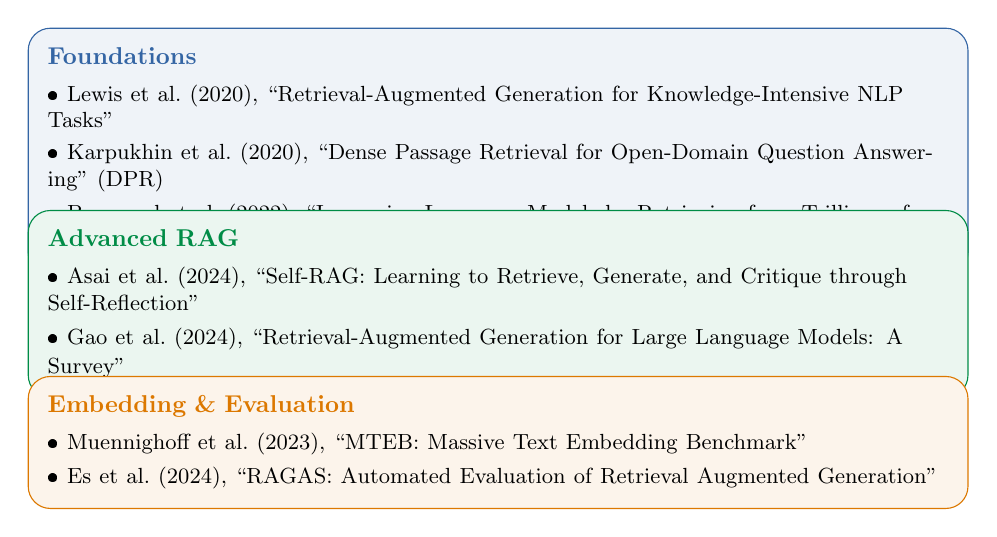
\begin{tikzpicture}[scale=0.88, transform shape]
  \node[draw=popblue, fill=popblue!8, rounded corners=8pt, text width=13cm, align=left, inner sep=8pt] at (0, 2.5) {
    \textbf{\textcolor{popblue}{Foundations}}\\[4pt]
    {\small
    \textbullet~Lewis et al.\ (2020), ``Retrieval-Augmented Generation for Knowledge-Intensive NLP Tasks''\\[2pt]
    \textbullet~Karpukhin et al.\ (2020), ``Dense Passage Retrieval for Open-Domain Question Answering'' (DPR)\\[2pt]
    \textbullet~Borgeaud et al.\ (2022), ``Improving Language Models by Retrieving from Trillions of Tokens'' (RETRO)
    }
  };
  \node[draw=paramgreen, fill=paramgreen!8, rounded corners=8pt, text width=13cm, align=left, inner sep=8pt] at (0, 0.3) {
    \textbf{\textcolor{paramgreen}{Advanced RAG}}\\[4pt]
    {\small
    \textbullet~Asai et al.\ (2024), ``Self-RAG: Learning to Retrieve, Generate, and Critique through Self-Reflection''\\[2pt]
    \textbullet~Gao et al.\ (2024), ``Retrieval-Augmented Generation for Large Language Models: A Survey''
    }
  };
  \node[draw=orange1, fill=orange1!8, rounded corners=8pt, text width=13cm, align=left, inner sep=8pt] at (0, -1.7) {
    \textbf{\textcolor{orange1}{Embedding \& Evaluation}}\\[4pt]
    {\small
    \textbullet~Muennighoff et al.\ (2023), ``MTEB: Massive Text Embedding Benchmark''\\[2pt]
    \textbullet~Es et al.\ (2024), ``RAGAS: Automated Evaluation of Retrieval Augmented Generation''
    }
  };
\end{tikzpicture}
\end{center}
\end{frame}

% ============================================================
% QUESTIONS
% ============================================================
\begin{frame}
\begin{center}
\vspace{2cm}
{\Huge\color{popblue}\textbf{Questions?}}

\vspace{1.5cm}
{\large Next: Hallucination \& Grounding}
\end{center}
\end{frame}

\end{document}
